\documentclass{beamer}
%\usepackage{beamerthemesplit} 
\usepackage{tikz}
\usetikzlibrary{trees}

\title{Computational Physics Group Project: \\ Ecosystem: predator and prey}
\author{David Hicks\\ Weiyao Ke \\ Shagun Maheshwari \\ Fan Zhang}
\date{\today}

\begin{document}

\frame{\titlepage}
\section[Outline]{Outline}
\frame{\tableofcontents}

\section{Introduction to eco-system modeling}
\frame
{
	\frametitle{What are Predator Prey models and where are they used?}
	
Systems involving competitive interaction of two "species" are some form of predator prey systems. \\
\begin{figure}[H]
  	\centering
      
	
\includegraphics[width = 0.2\textwidth]{./pics/resource_consumer.jpeg} 
        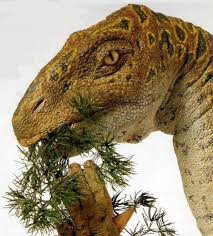
\includegraphics[width = 0.25\textwidth]{./pics/Plant_herbivore.jpeg} 
        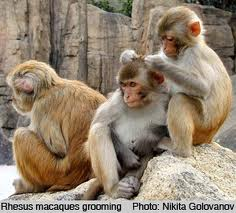
\includegraphics[width = 0.31\textwidth]{./pics/Parasite_host.jpeg} 
       
        \label{Intro}
  \end{figure}

They deal with the general loss-win interactions and hence may have applications outside of ecosystems. 
}

\frame
{
 	\frametitle{Population interaction of predator and prey in eco-system}
 
	\begin{figure}[htbp]
	\begin{center}
		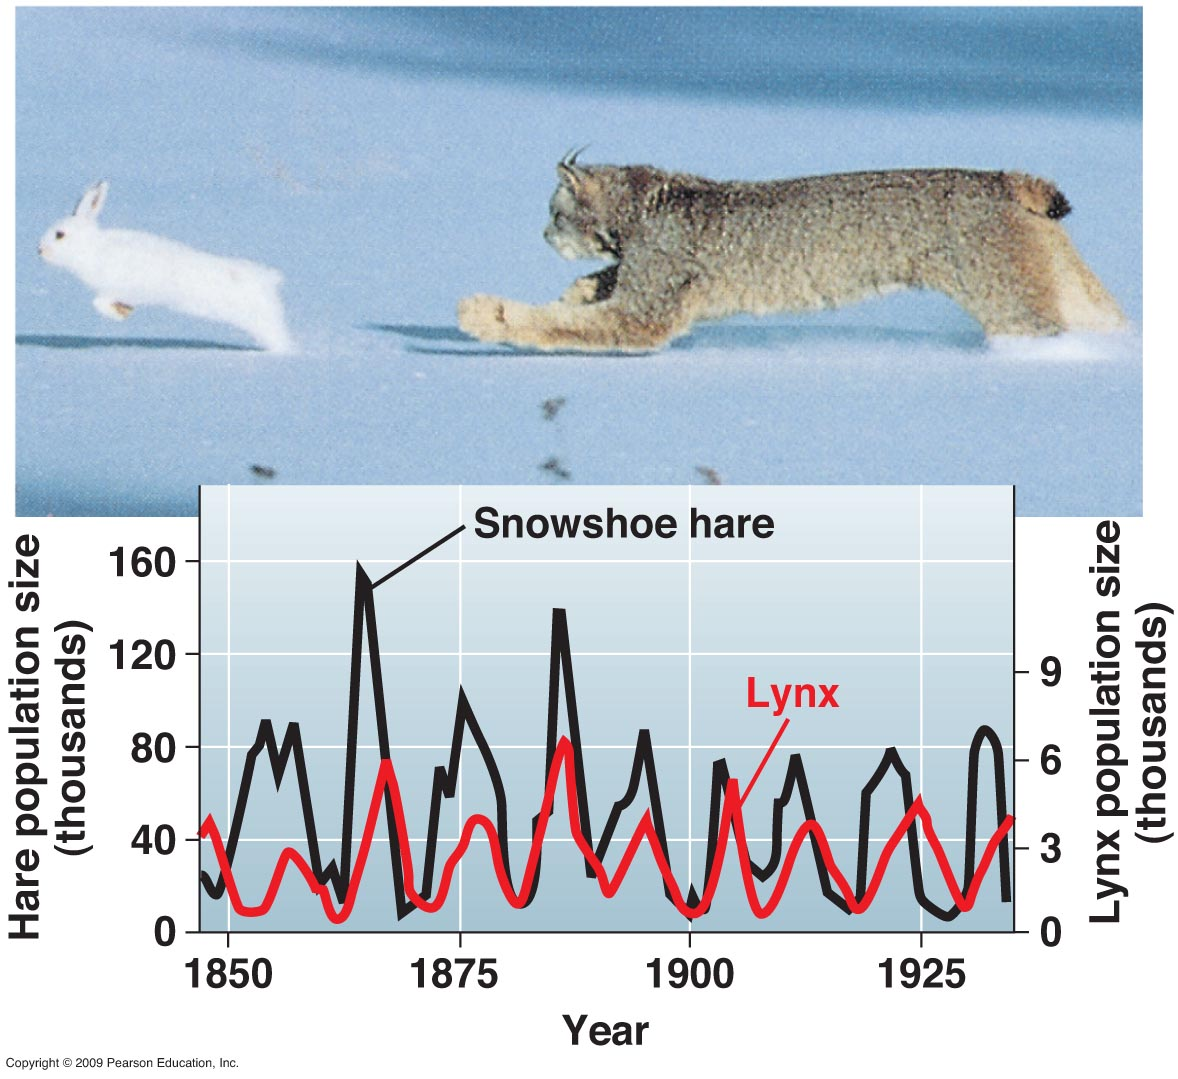
\includegraphics[width=0.4\textwidth]{./pics/predator_prey2.jpeg}
	\caption{http://www.anselm.edu/homepage/jpitocch/genbi101/ecology1intropops.html}
	\label{default}
	\end{center}
	\end{figure} 
}

\frame
{
 	\frametitle{A simplified deterministic mode: L-V equation}
 	The dynamics of biological systems consist of one predator and one prey can be described by Lotka-Volterra (LV) equations:
 	\begin{eqnarray*}
 	\frac{dx}{dt} &=& \alpha x - \beta x y = x(\alpha - \beta y) \\
 	\frac{dy}{dt} &=& - \gamma y + \delta x y = - y (\gamma - \delta x)
 	\end{eqnarray*}
    Where, x is the number of prey, y is the number of predator, $\frac{dx}{dt}$ and $\frac{dy}{dt}$ represent the growth rates of two populations, and $\alpha, \beta, \gamma$ and $\delta$ are parameters describing the interaction of two species. \\
}

\frame
{
    \frametitle{A simplified deterministic mode: L-V equation}
     When the biological system has reached eco-equilibrium, the number of predator and prey are supposed to be either situation below.
    \begin{itemize}
    \item 1. $x = 0, y = 0$: Both species extinct. 
    \item 2. $x = \frac{\gamma}{\delta}, y = \frac{\alpha}{\beta}$: Predator and Prey reach a periodic stable situation. The number of animals evolve in a sinusoidal way.
    \end{itemize}
    \medskip \medskip
 	Disadvantage: number of species, limit of interaction. \\
    Advanced model: competitive L-V equation for trophic interaction; generalized L-V equation for multiple species.
}

\section{Simulation and Implementation}
\frame
{
 	 \frametitle{Simulation of a eco-system with predator and prey}
  	A simulation keep the essential nature of the interaction between and within the species, and predict the 	evolution of population step by step.
  	\begin{itemize}
  	\item<1->{Both predator and prey reproduces when they reach the age of reproduction}
  	\item<2->{Predator feeds on prey.}
  	\item<3->{Predator and prey will die out if maximum age is reached or starved for enough long time}
  	\item<4->{However, simulation is a random process and change the deterministic nature of LV equation (more realistic).}
  	\end{itemize} 
}

\frame
{
 	\frametitle{Structural setup}

	\tikzstyle{every node}=[anchor=west]
	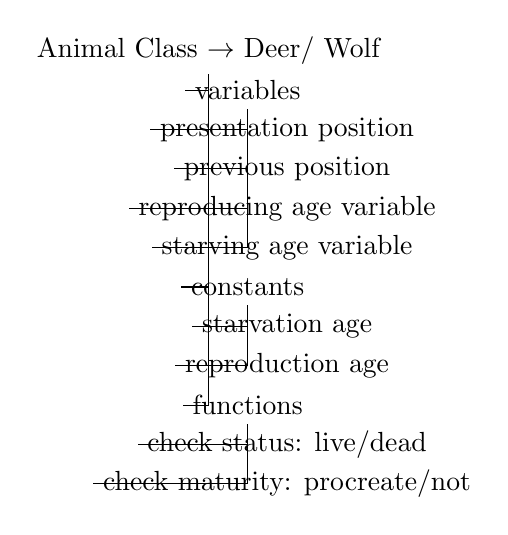
\begin{tikzpicture}
	[grow via three points={one child at (0.5,-0.5) and two children at (0.5,-0.5) and (0.5,-1)}, edge from parent path={(\tikzparentnode.south) |- (\tikzchildnode.west)}]
 	 \node {Animal Class $\rightarrow$ Deer/ Wolf}
    	child{ node{variables}
    	     	child { node {presentation position}}		
   		child { node {previous position}}
    		child { node {reproducing age variable}}
    		child { node {starving age variable}}
    		}
    	child [missing] {}				
    	child [missing] {}				
    	child [missing] {}	
    	child [missing] {}	
    	child{ node{constants}
    		child { node {starvation age}}
    		child { node {reproduction age}}
		}
   	 child [missing] {}	
    	child [missing] {}	
   	 child{ node{functions}
    		child { node {check status: live/dead}}
    		child { node {check maturity: procreate/not}}
		};		
	\end{tikzpicture}
}

\frame
{
 	 \frametitle{Structural setup of the code}

	\tikzstyle{every node}=[anchor=west]
	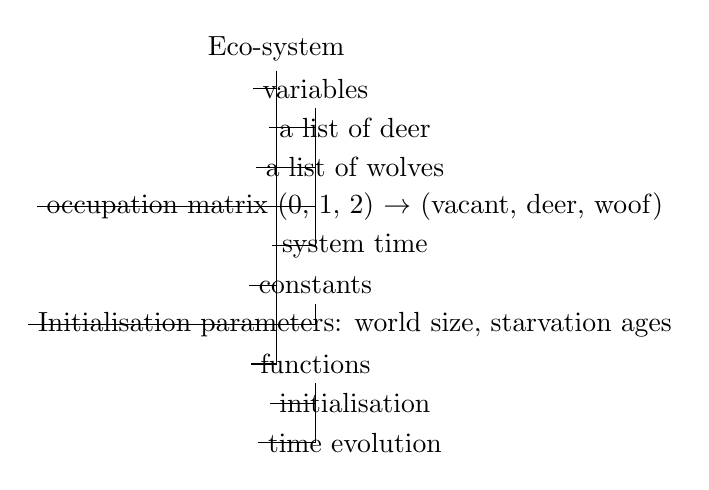
\begin{tikzpicture}
	[grow via three points={one child at (0.5,-0.5) and two children at (0.5,-0.5) and (0.5,-1)}, edge from parent path={(\tikzparentnode.south) |- (\tikzchildnode.west)}]
  	\node {Eco-system}
    	child{ node{variables}
    	     	child { node {a list of deer}}		
   		child { node {a list of wolves}}
		child { node {occupation matrix (0, 1, 2) $\rightarrow$ (vacant, deer, woof)}}
    		child { node {system time}}
    	}
    	child [missing] {}				
   	child [missing] {}				
    	child [missing] {}	
    	child [missing] {}
    	child{ node{constants}
    		child { node {Initialisation parameters: world size, starvation ages}}
	}
    	child [missing] {}	
    	child{ node{functions}
    		child { node {initialisation}}
    		child { node {time evolution}}
	};		
\end{tikzpicture}
}


\frame
{
  	\frametitle{Initialisation}
  	A sanity simulation requires several constrains on the initialisation of parameters.
  	\begin{itemize}
  	\item<1->{Reproduction age of predators must be larger than their starvation age. (Or else wolf can sustain themselves ...)}
  	\item<2->{Starvation age of the deer is extremely large. (Always enough plants!)}
	\item<3->{A realistic population always have some age structures, so we use a uniform initial age distribution for the animals.}
  	\end{itemize} 
}

\frame
{
  	\frametitle{Evolution of Wolves}
 	 We set up a $N \times N$ grid and simulate the eco-system with L-V equation. \\
  	 \begin{itemize}
  	\item<1->{Step $1$: check wolf and deer population, increase its age, and see whether a single animal has starved to death.}
  	\item<2->{Step $2$: evolution of wolves:
  
 	 \begin{figure}[htb]
  	\begin{center}
 	 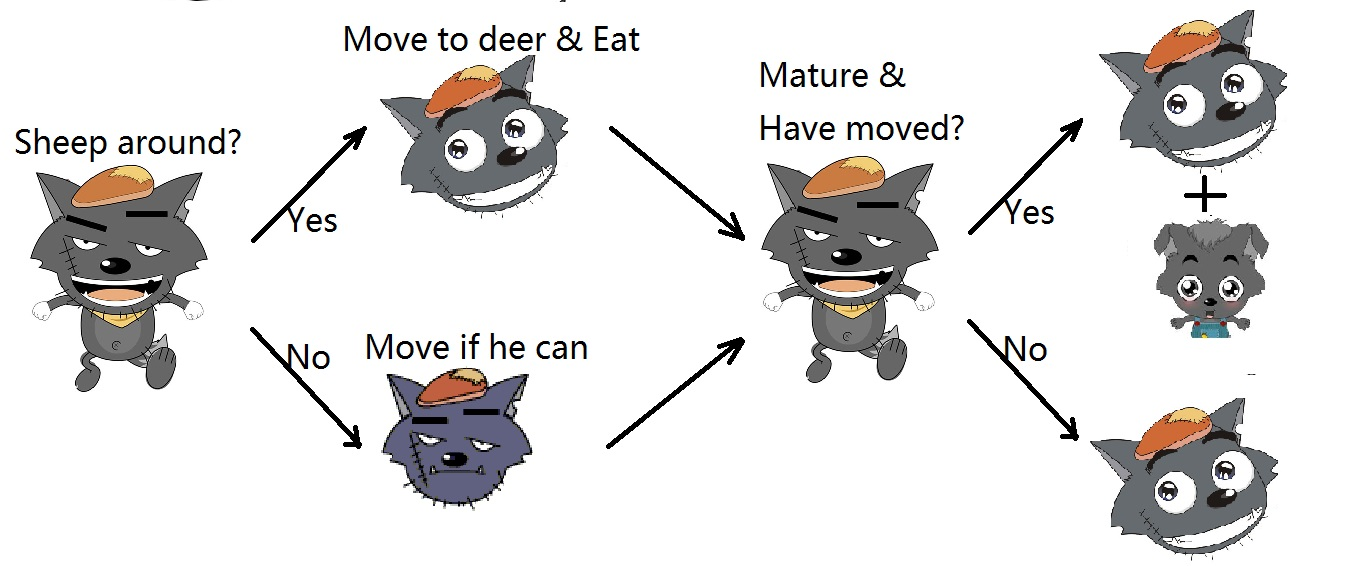
\includegraphics[width=\textwidth]{./pics/wolf.jpeg}
 	 \label{default}
  	\end{center}
  	\end{figure}
 	 }
 	 \end{itemize}
}

\frame
{
  	\frametitle{Evolution of deer}
  	Evolution of deers: \\
 	\begin{itemize}
  	\item<1->{Step 1: Delete all unfortunate deers.}
  	\item<2->{Setp 2: Evolution of live deers.
 
  	\begin{figure}[htbp]
 	 \begin{center}
  	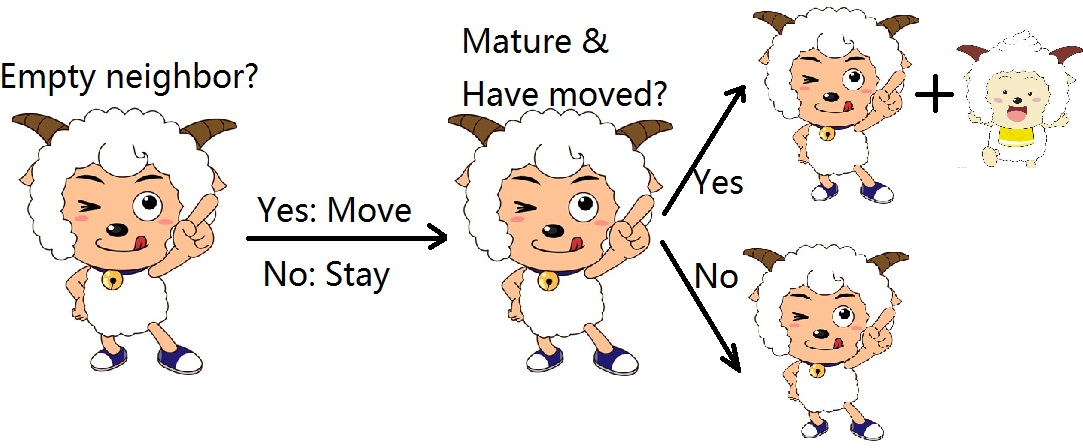
\includegraphics[width=\textwidth]{./pics/goat.jpeg}
  	\label{default}
 	 \end{center}
  	\end{figure}
  	}
   	\end{itemize}
}

\frame
{
	\frametitle{Population interaction of predator and prey in eco-system}

	\begin{figure}[htbp]
	\begin{center}
	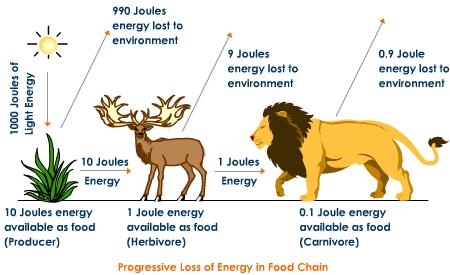
\includegraphics[width=1\textwidth]{./pics/progressive-energy-loss.jpeg}
	\caption{default}
	\label{default}
	\end{center}
	\end{figure}
}

\frame
{
	\frametitle{Generic results}

	\begin{figure}[htbp]
	\begin{center}
	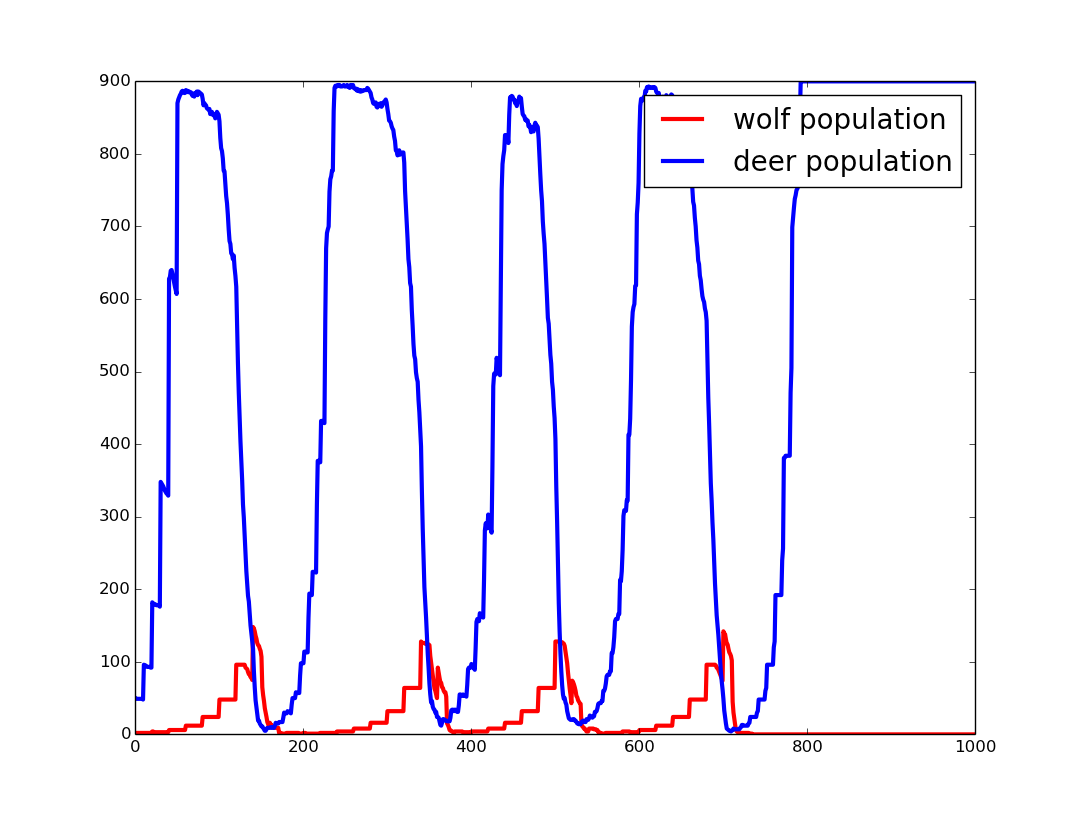
\includegraphics[width=0.6\textwidth]{./pics/age_structure.png}
	\caption{Initialised without age structure. This is an example of wolf distinction.}
	\label{default}
	\end{center}
	\end{figure}
}

\frame
{
	\frametitle{Generic results}

	\begin{figure}[htbp]
	\begin{center}
	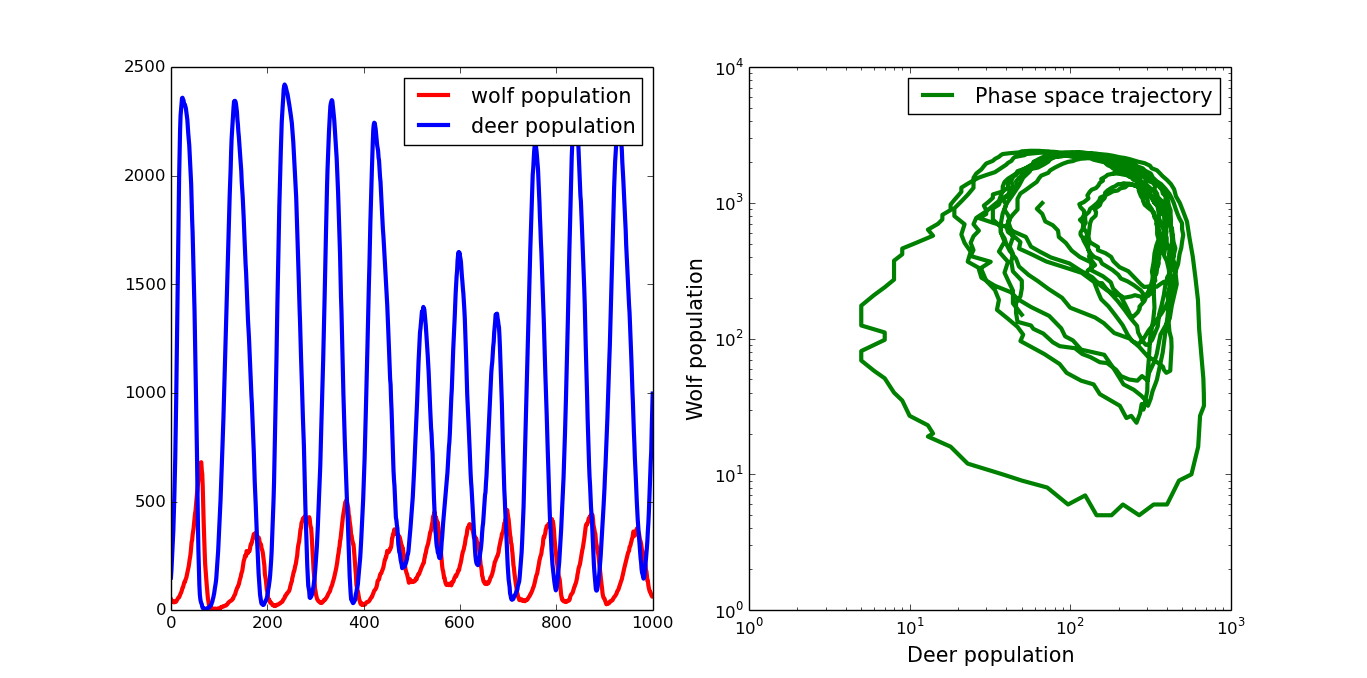
\includegraphics[width=0.8\textwidth]{./pics/phase_space.png}
	\caption{Initialised with uniform age structure. A quasi-periodic evolution is obtained.}
	\label{default}
	\end{center}
	\end{figure}
}

\frame
{
  \frametitle{Parameter Search}
  \underline{5 parameters to test (5-D parameter space)}
  \begin{itemize}
  \item{\textbf{Initial population of deer}}
  \item{\textbf{Initial population of wolves}}
  \item{Reproduction age of deer}
  \item{Reproduction age of wolf}
  \item{Starvation "age" of wolf}
  \end{itemize} 

  \underline{Reduce to 4 dimensions (4-D)}
  \begin{itemize}
  \item{\textbf{Ratio of initial populations : Size of point}}
  \item{Reproduction age of deer : x-axis}
  \item{Reproduction age of wolf : y-axis}
  \item{Starvation "age" of wolf : z-axis}
  \end{itemize} 

}
\frame
{
  \frametitle{Results of Full Parameter Search}
  \begin{figure}[H]
	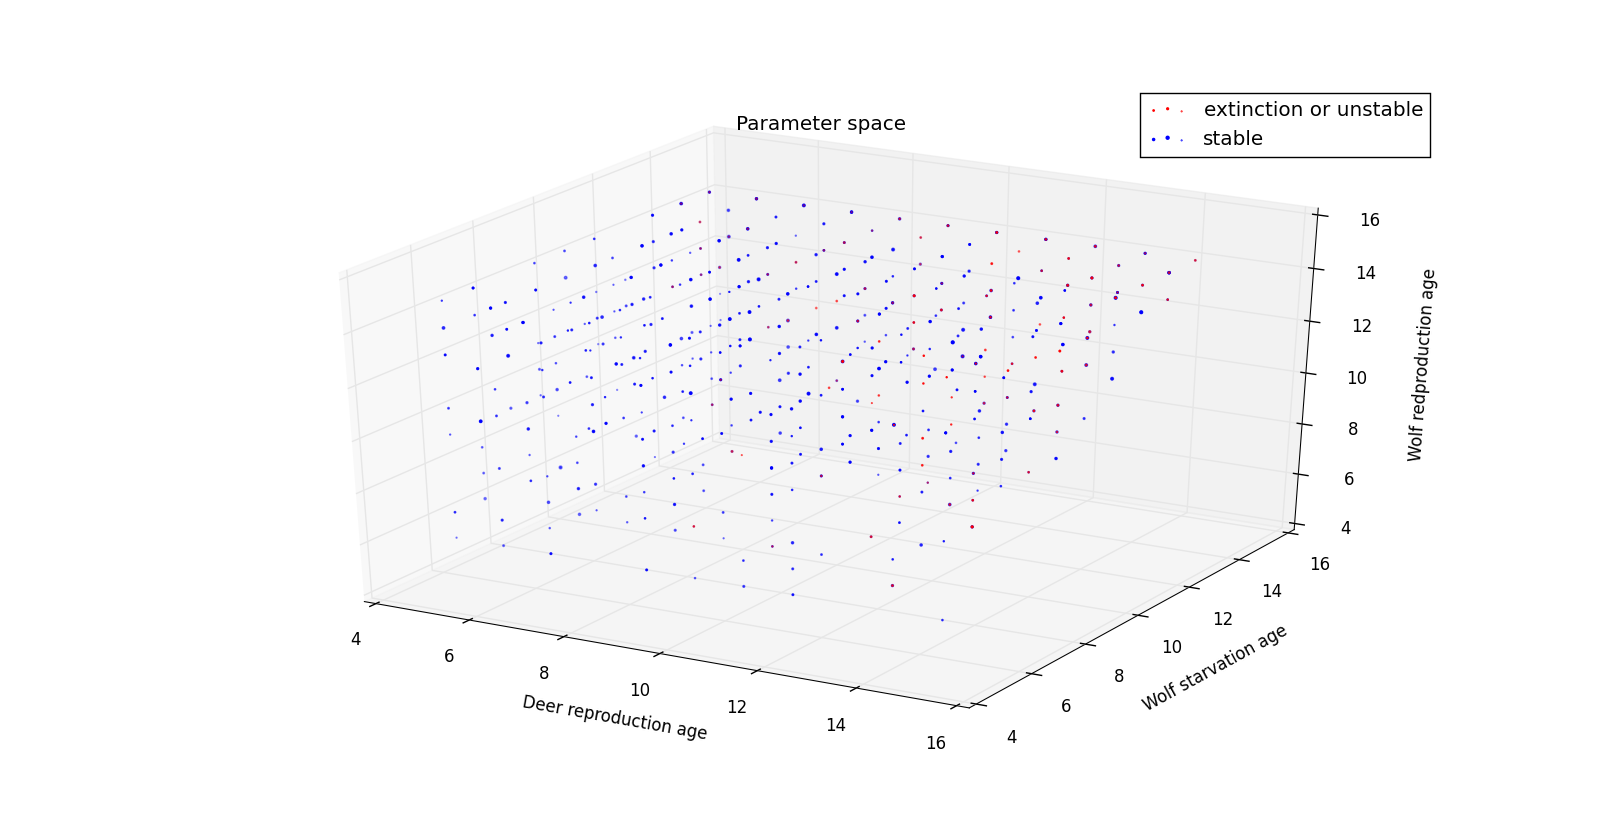
\includegraphics[width = 1\textwidth]{./pics/Eco_All_param_front.png} 
  \end{figure}
        
}

\frame
{
  \frametitle{Results of Full Parameter Search}
  \begin{figure}[H]
	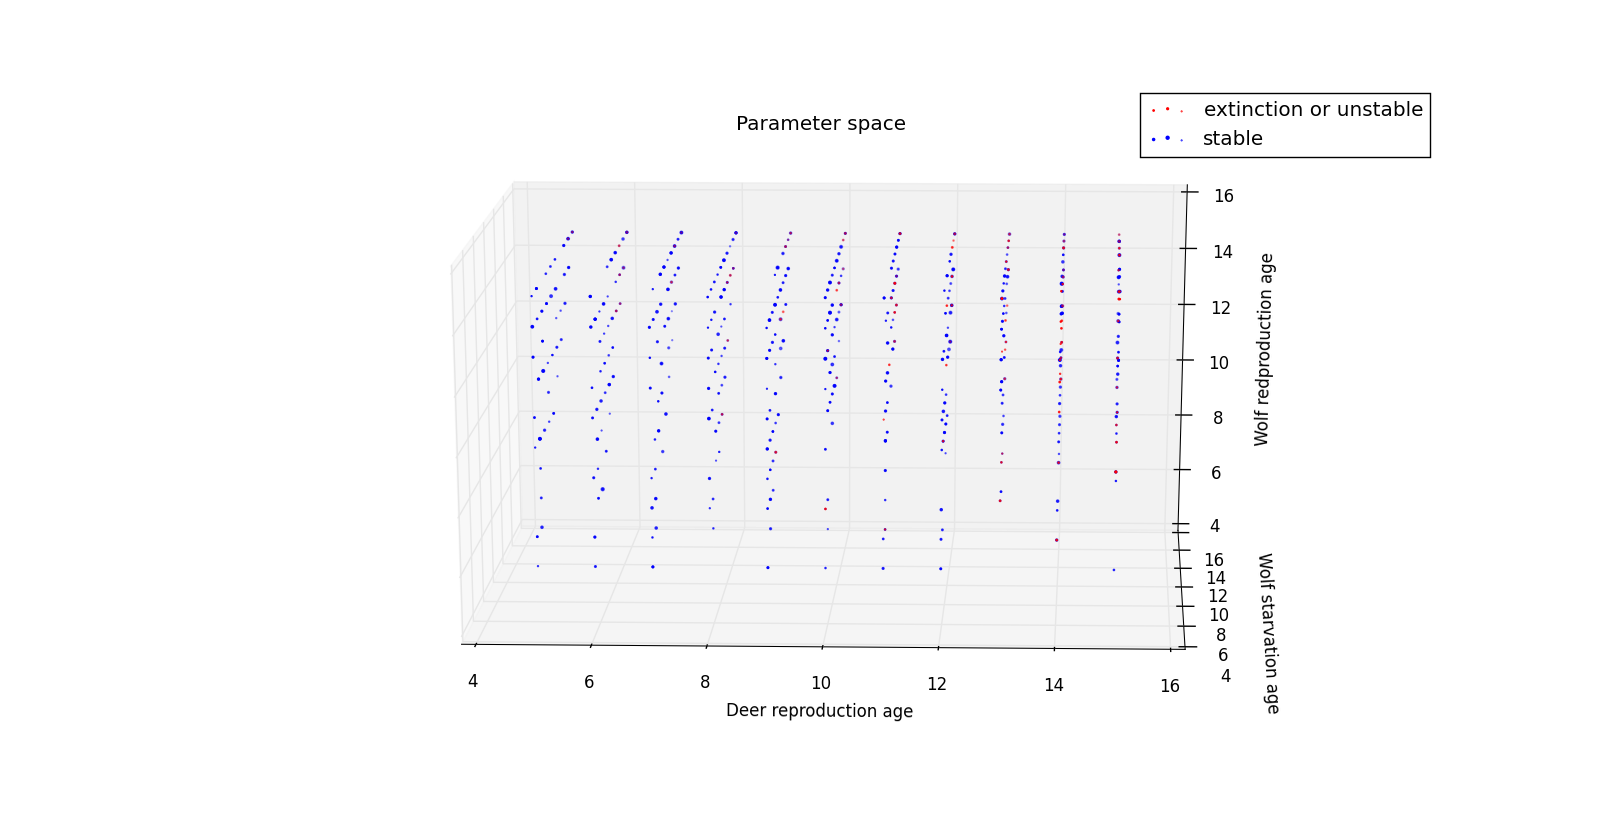
\includegraphics[width = 1\textwidth]{./pics/Eco_All_param_rep_v_rep.png} 
  \end{figure}
}

\frame
{
  \frametitle{Results of Full Parameter Search}
  \begin{figure}[H]
	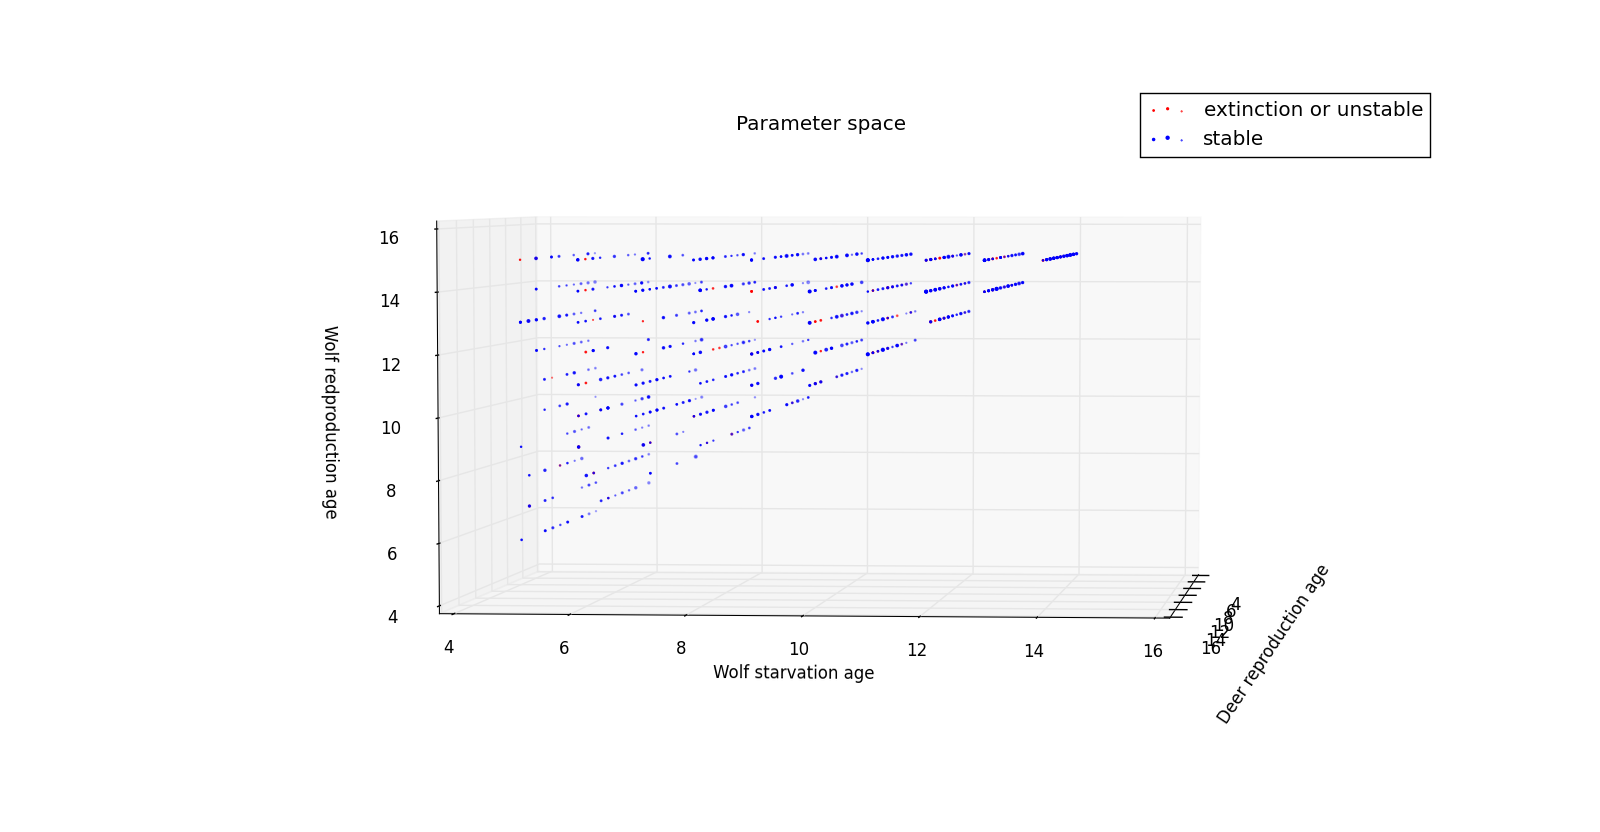
\includegraphics[width = 1\textwidth]{./pics/Eco_All_param_wage_v_wstarve.png}
  \end{figure}
}
                
\frame
{
  \frametitle{Results of Full Parameter Search}
  \begin{figure}[H]
	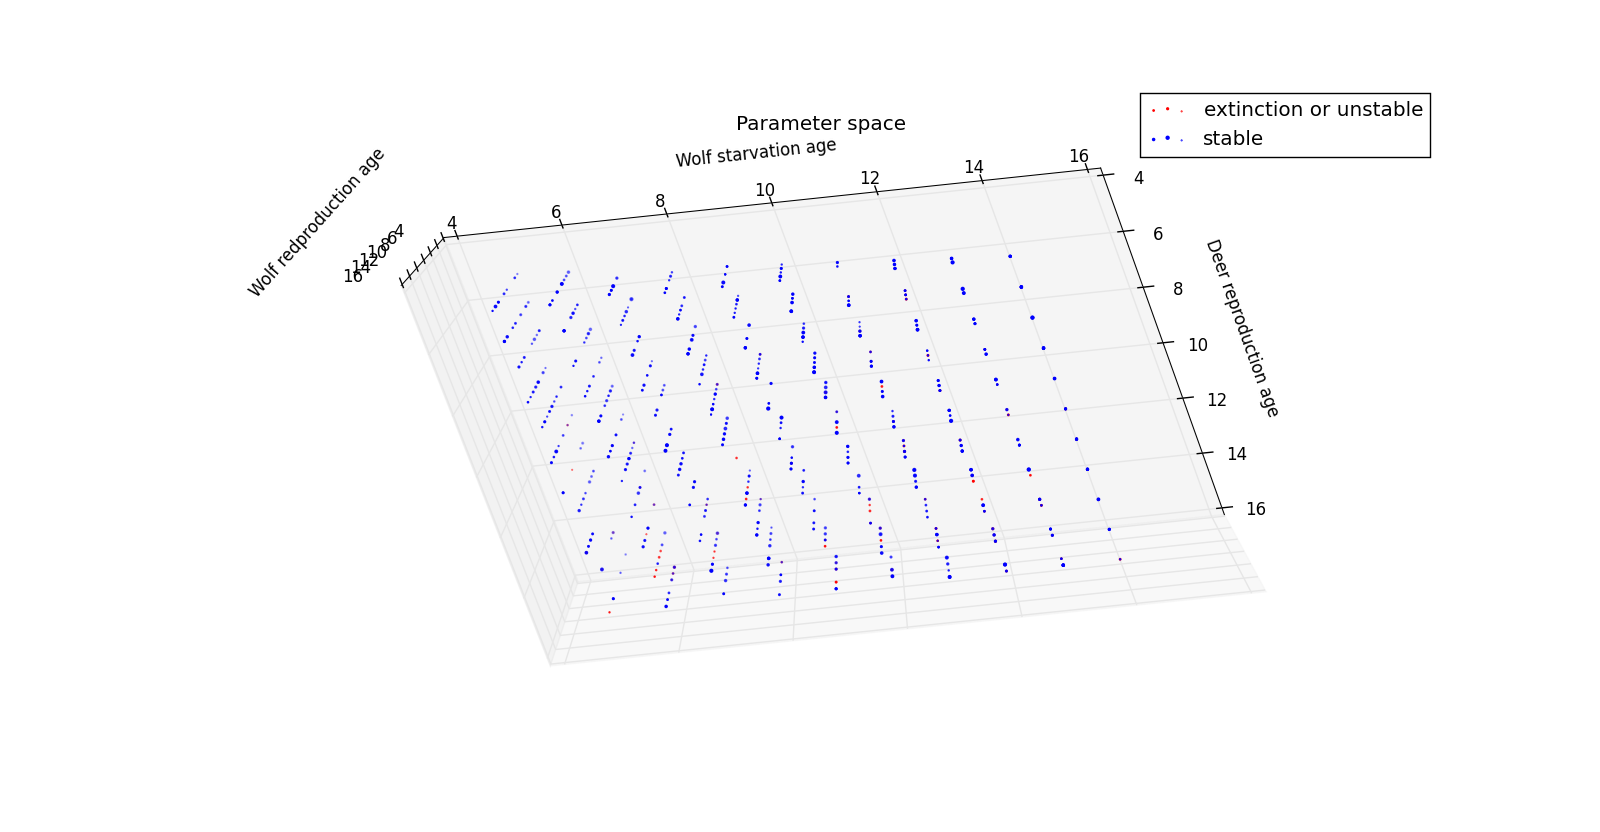
\includegraphics[width = 1\textwidth]{./pics/Eco_All_param_wstarve_v_drep.png}
  \end{figure}

}


\frame
{
  \frametitle{Results of Full Parameter Search}
  \begin{figure}[H]
        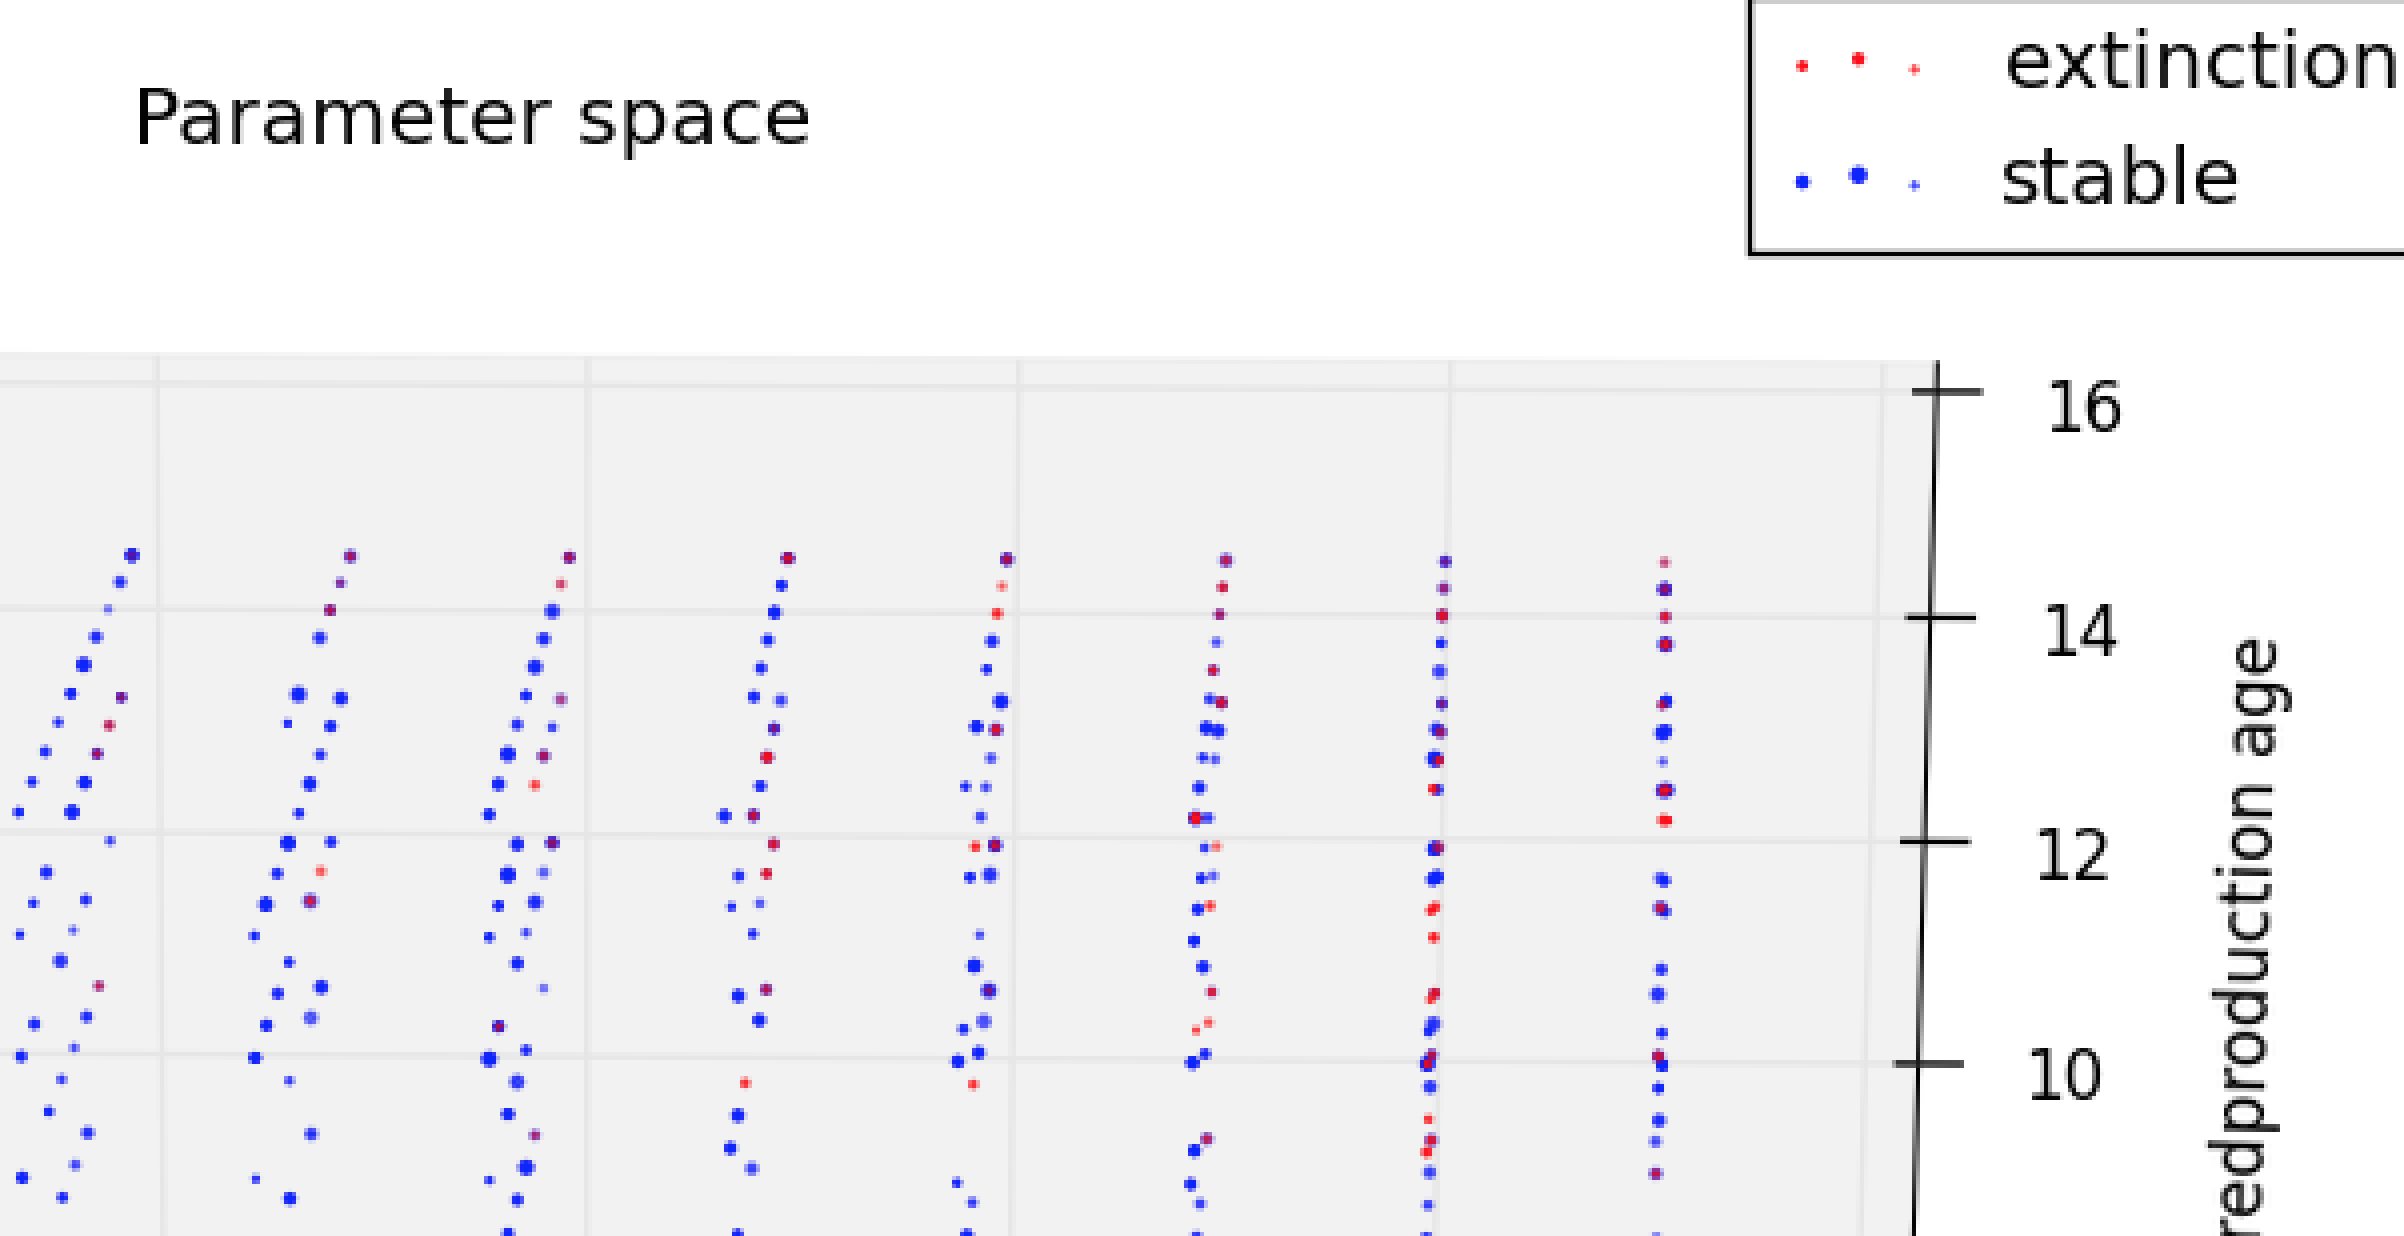
\includegraphics[width = 1\textwidth]{./pics/Zoomedin_3D.png}
  \end{figure}
}

\frame
{
	\frametitle{Results of Full Parameter Search}
	  The following is an excerpt from the paper, "A. K. Dewdney, Computer Recreations"  :
	  \begin{figure}[H]
  		\centering
		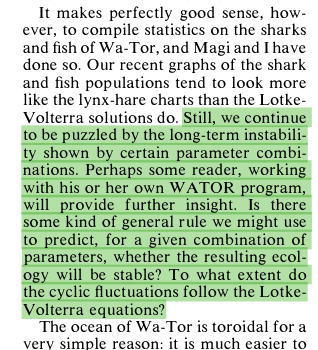
\includegraphics[width = 0.5\textwidth]{./pics/paper_predatorprey.png}
        \label{refpaper}
  \end{figure}

}

\frame
{
  \frametitle{Results of Restricted Parameter Search}
  \center{Fix initial population ratios}
  \begin{figure}[H]
  \centering
        \begin{tabular}{@{}cc@{}cc@{}cc@{}}
                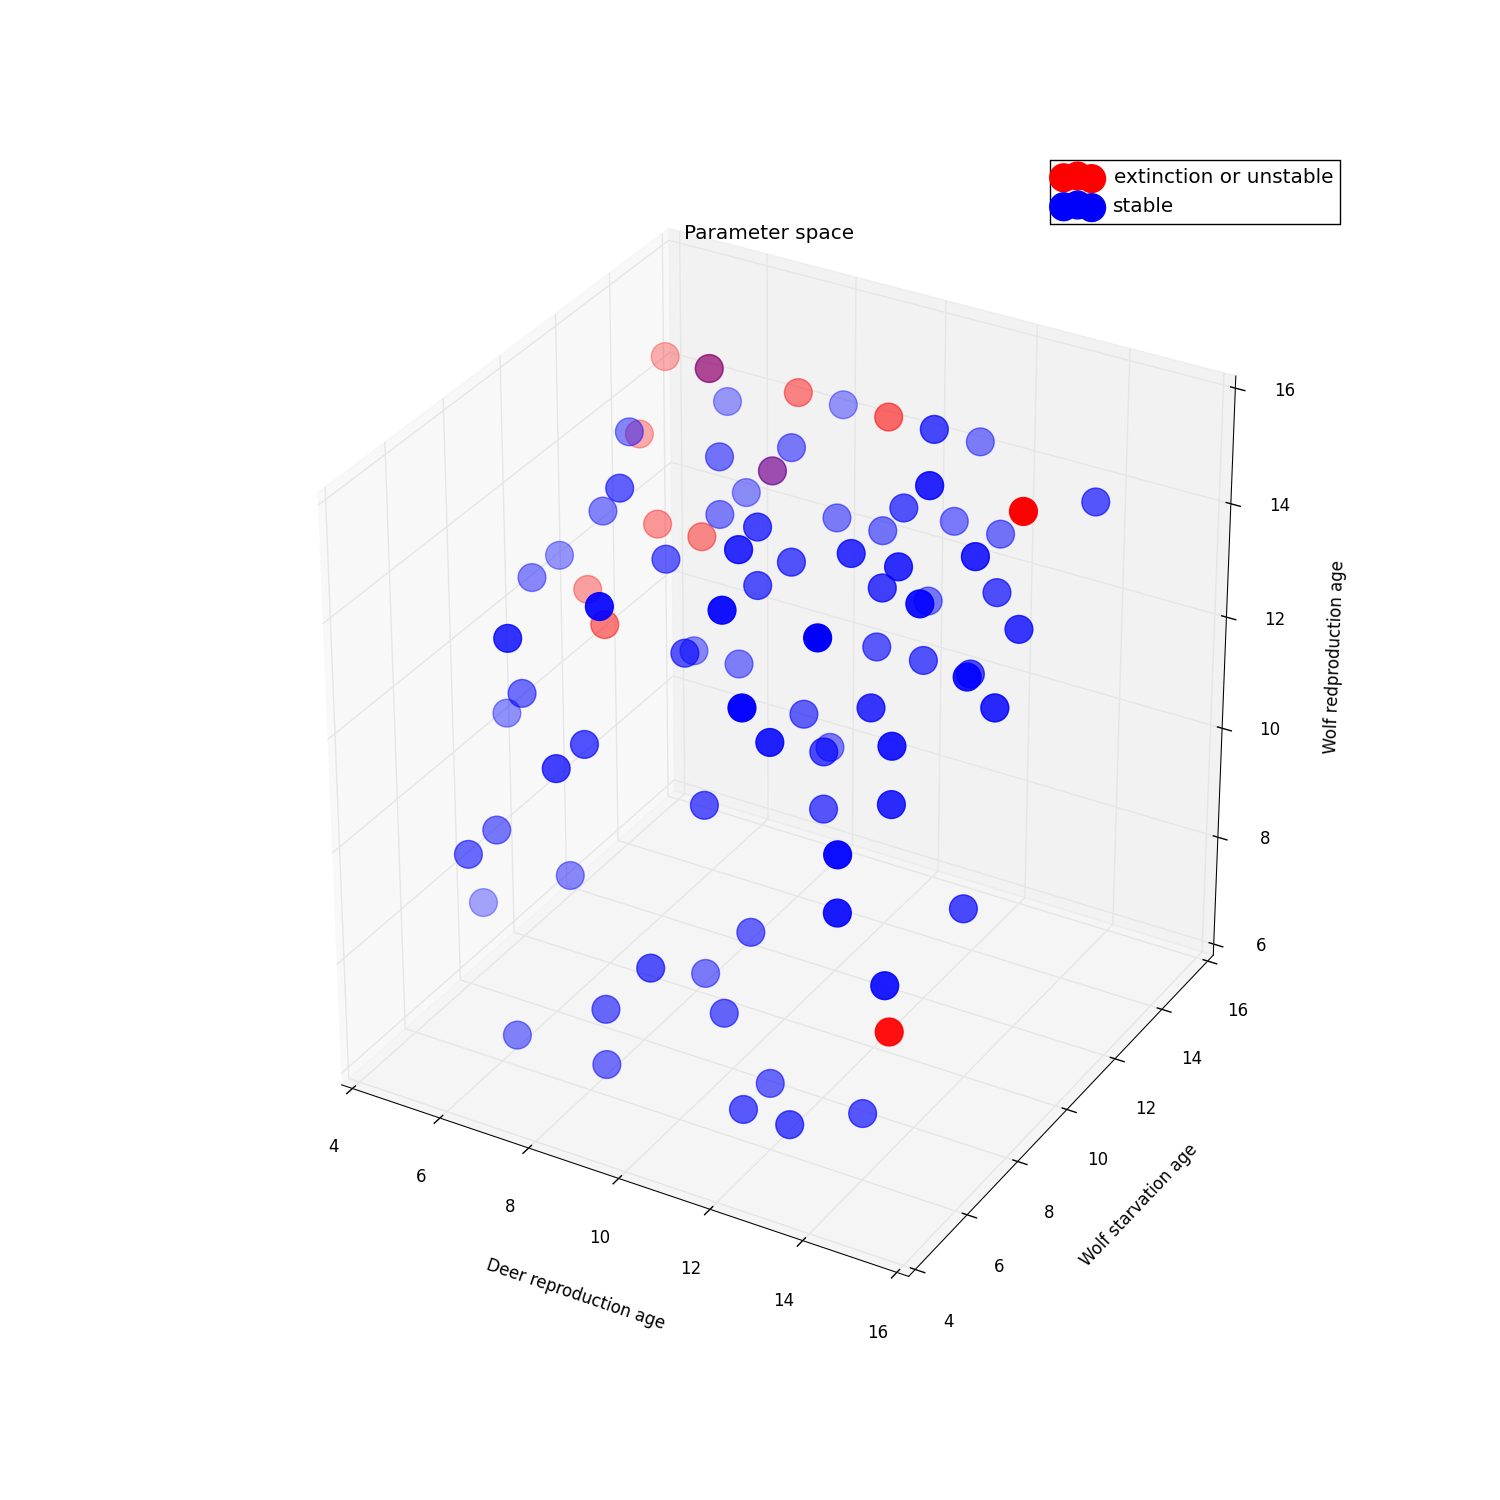
\includegraphics[width = 0.3\textwidth]{./pics/Restricted_Parameter_space_d2500_w250.png} &
                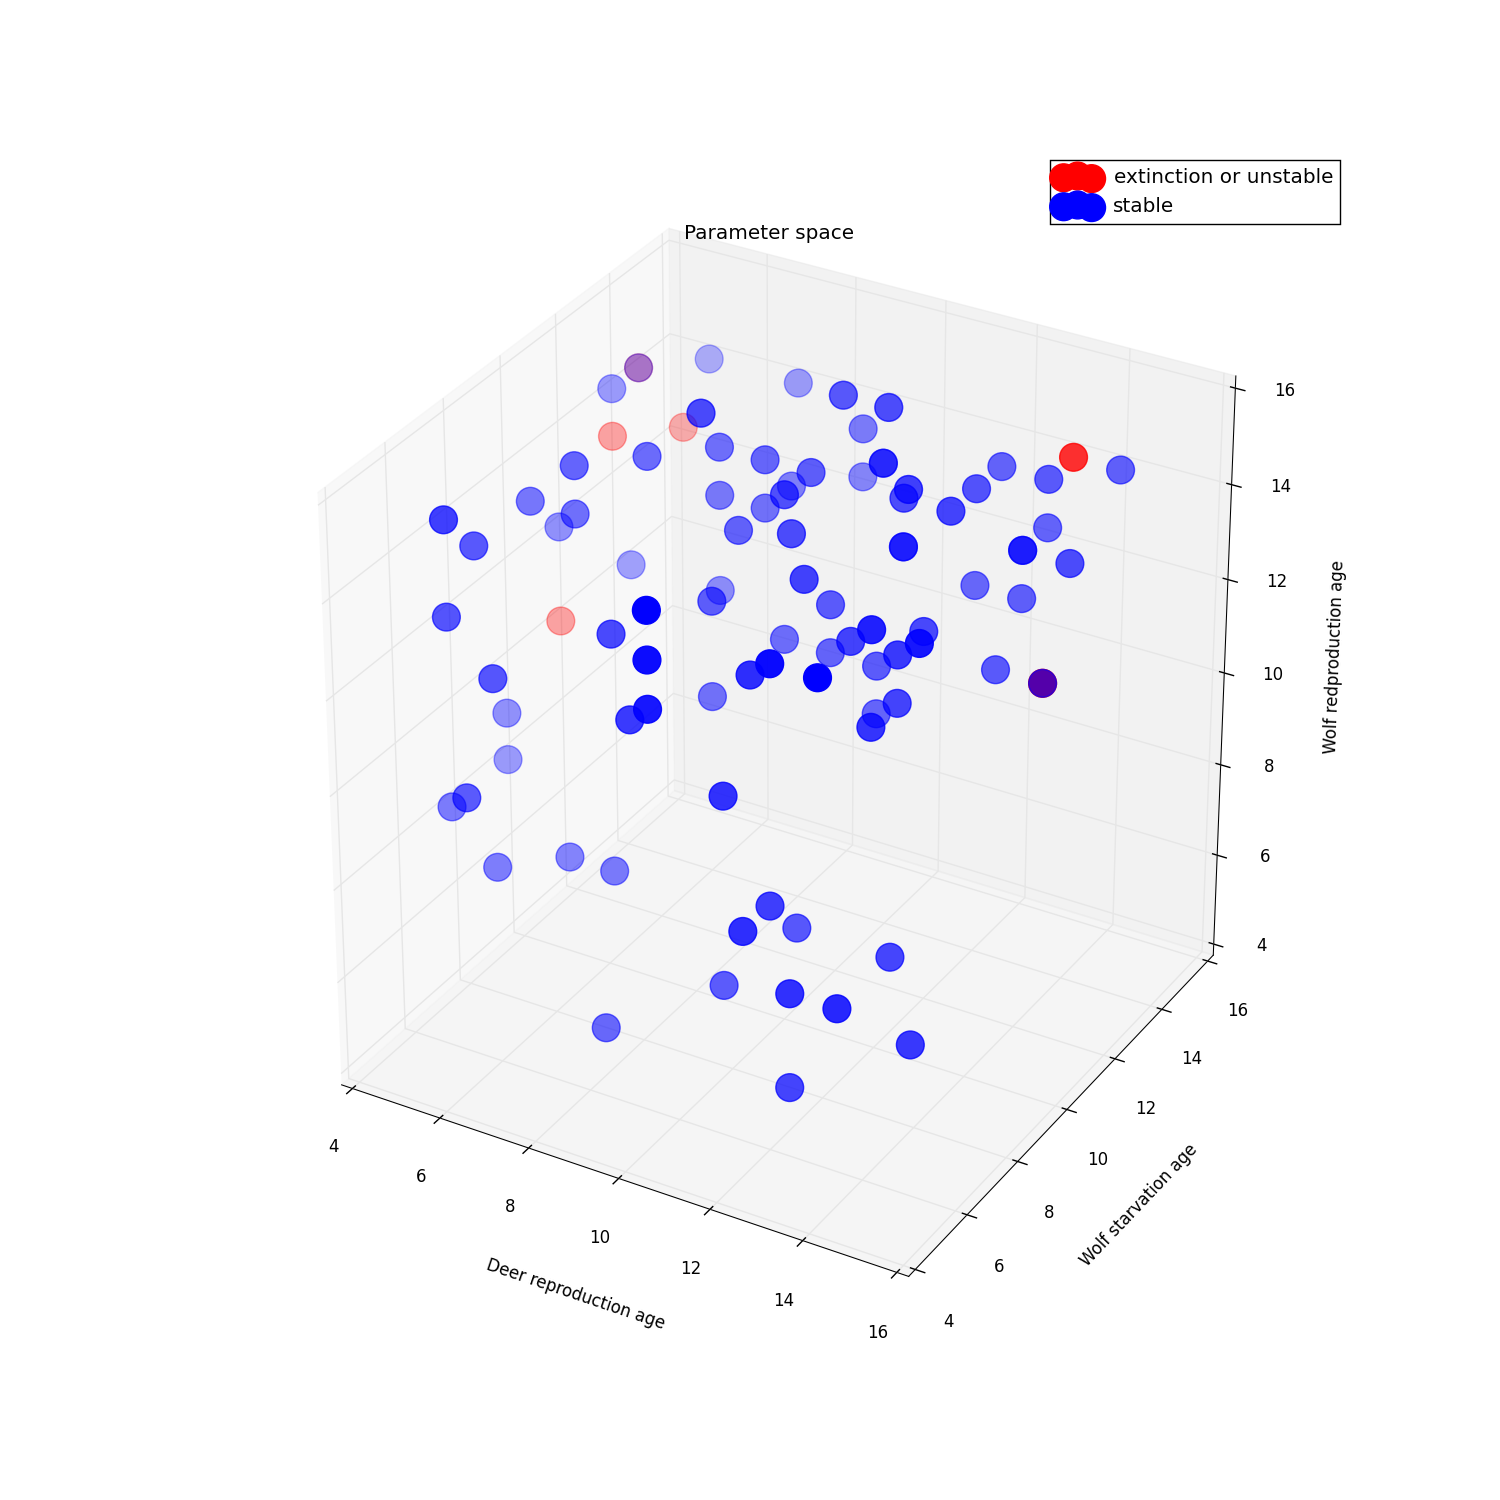
\includegraphics[width = 0.3\textwidth]{./pics/Restricted_Parameter_space_d3000_w500.png} &
                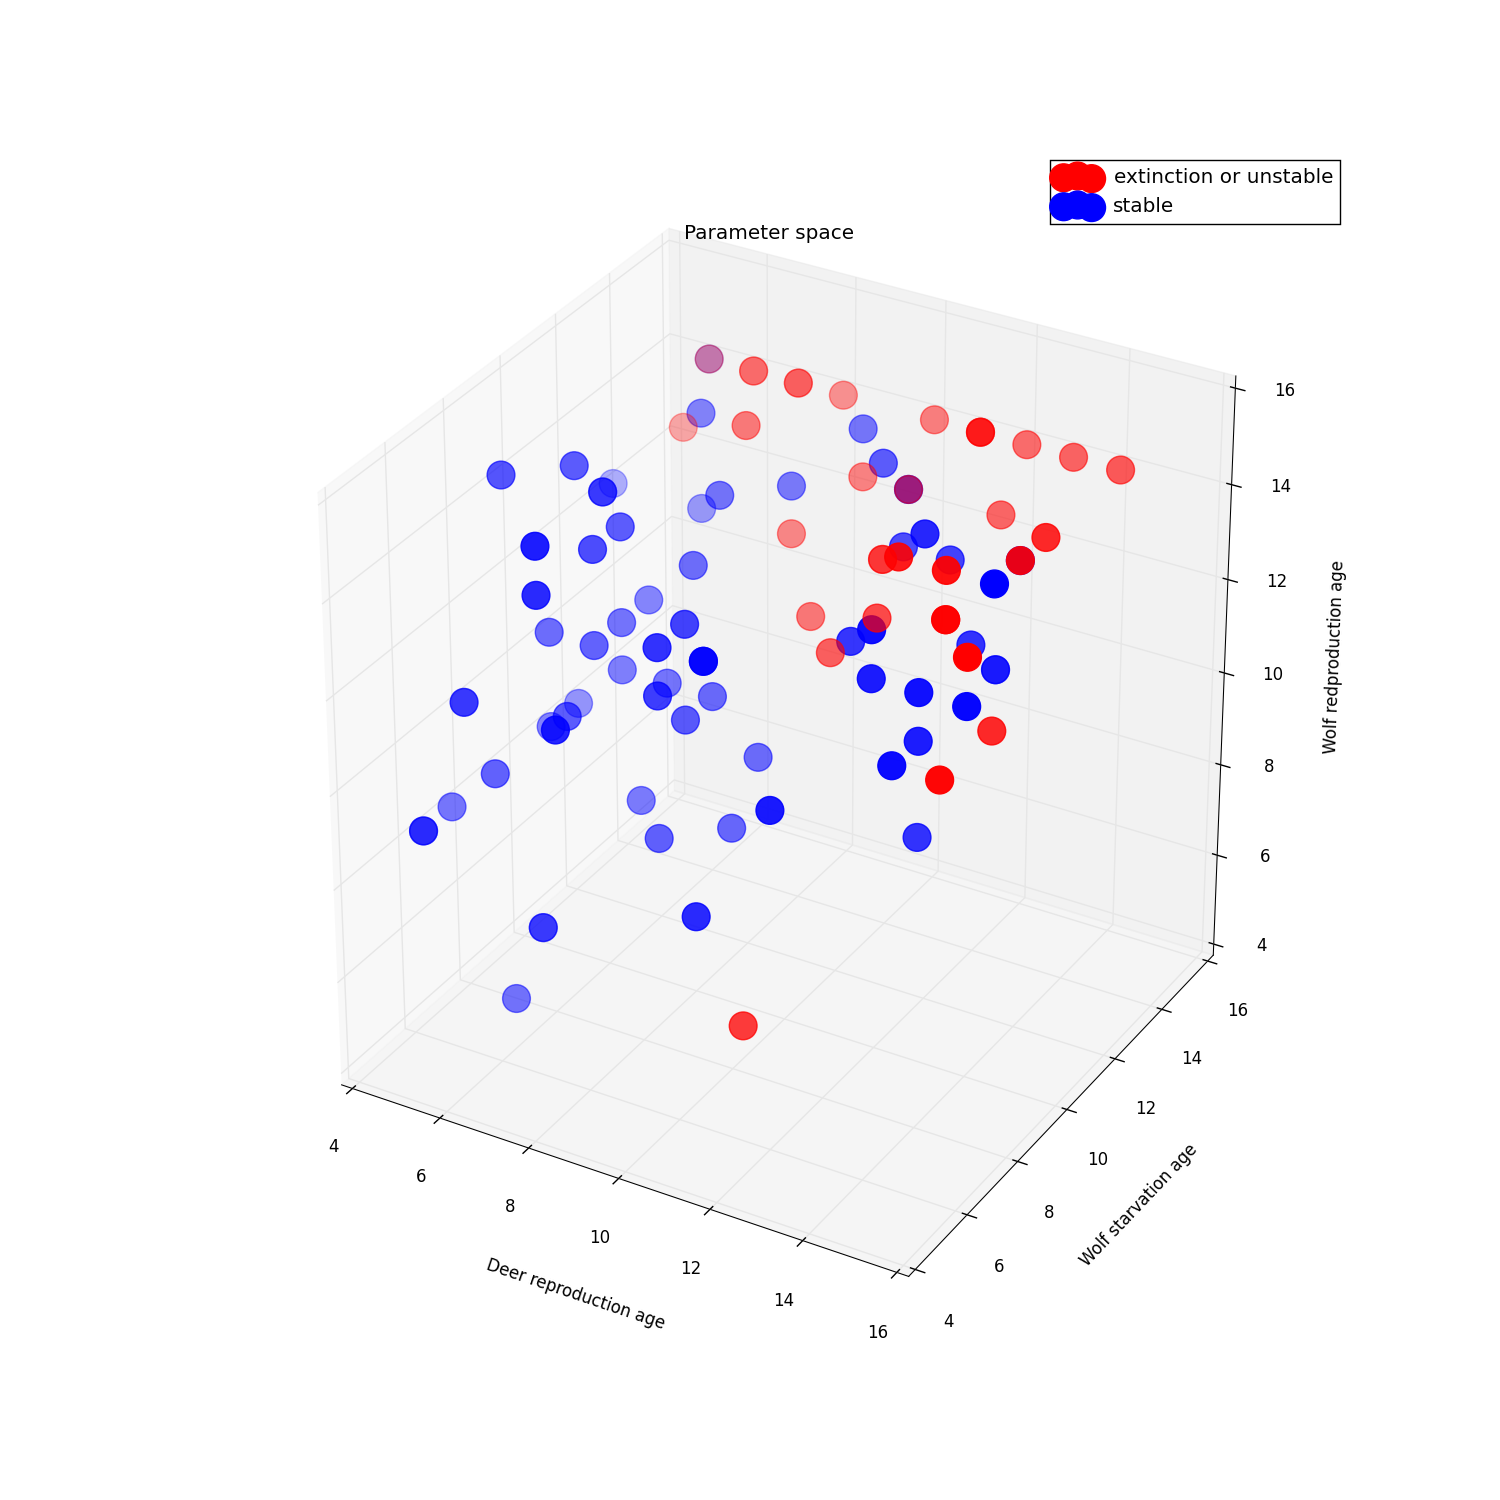
\includegraphics[width = 0.3\textwidth]{./pics/Restricted_Parameter_space_d2000_w2000.png} \\
                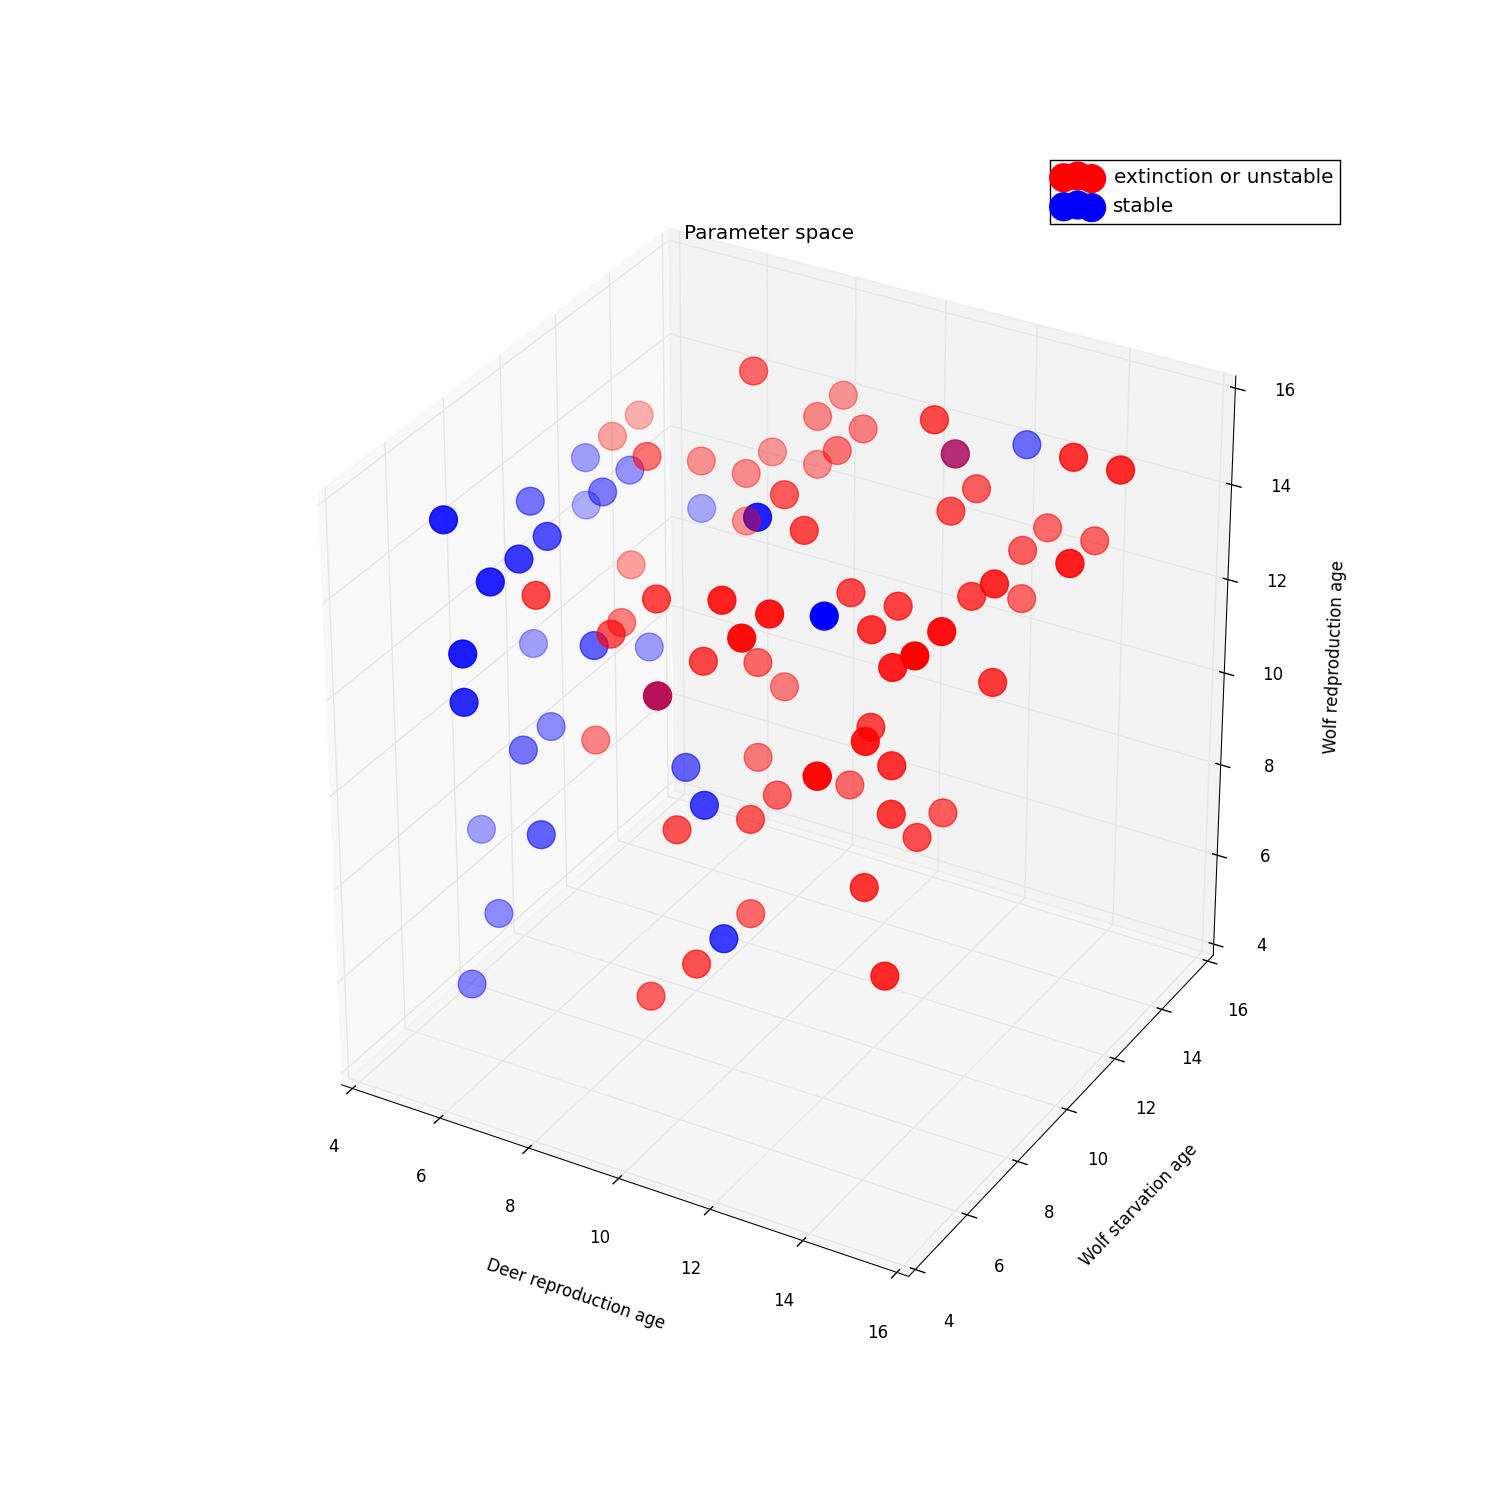
\includegraphics[width = 0.2\textwidth]{./pics/Restricted_Parameter_space_d500_w3000.png} &&
		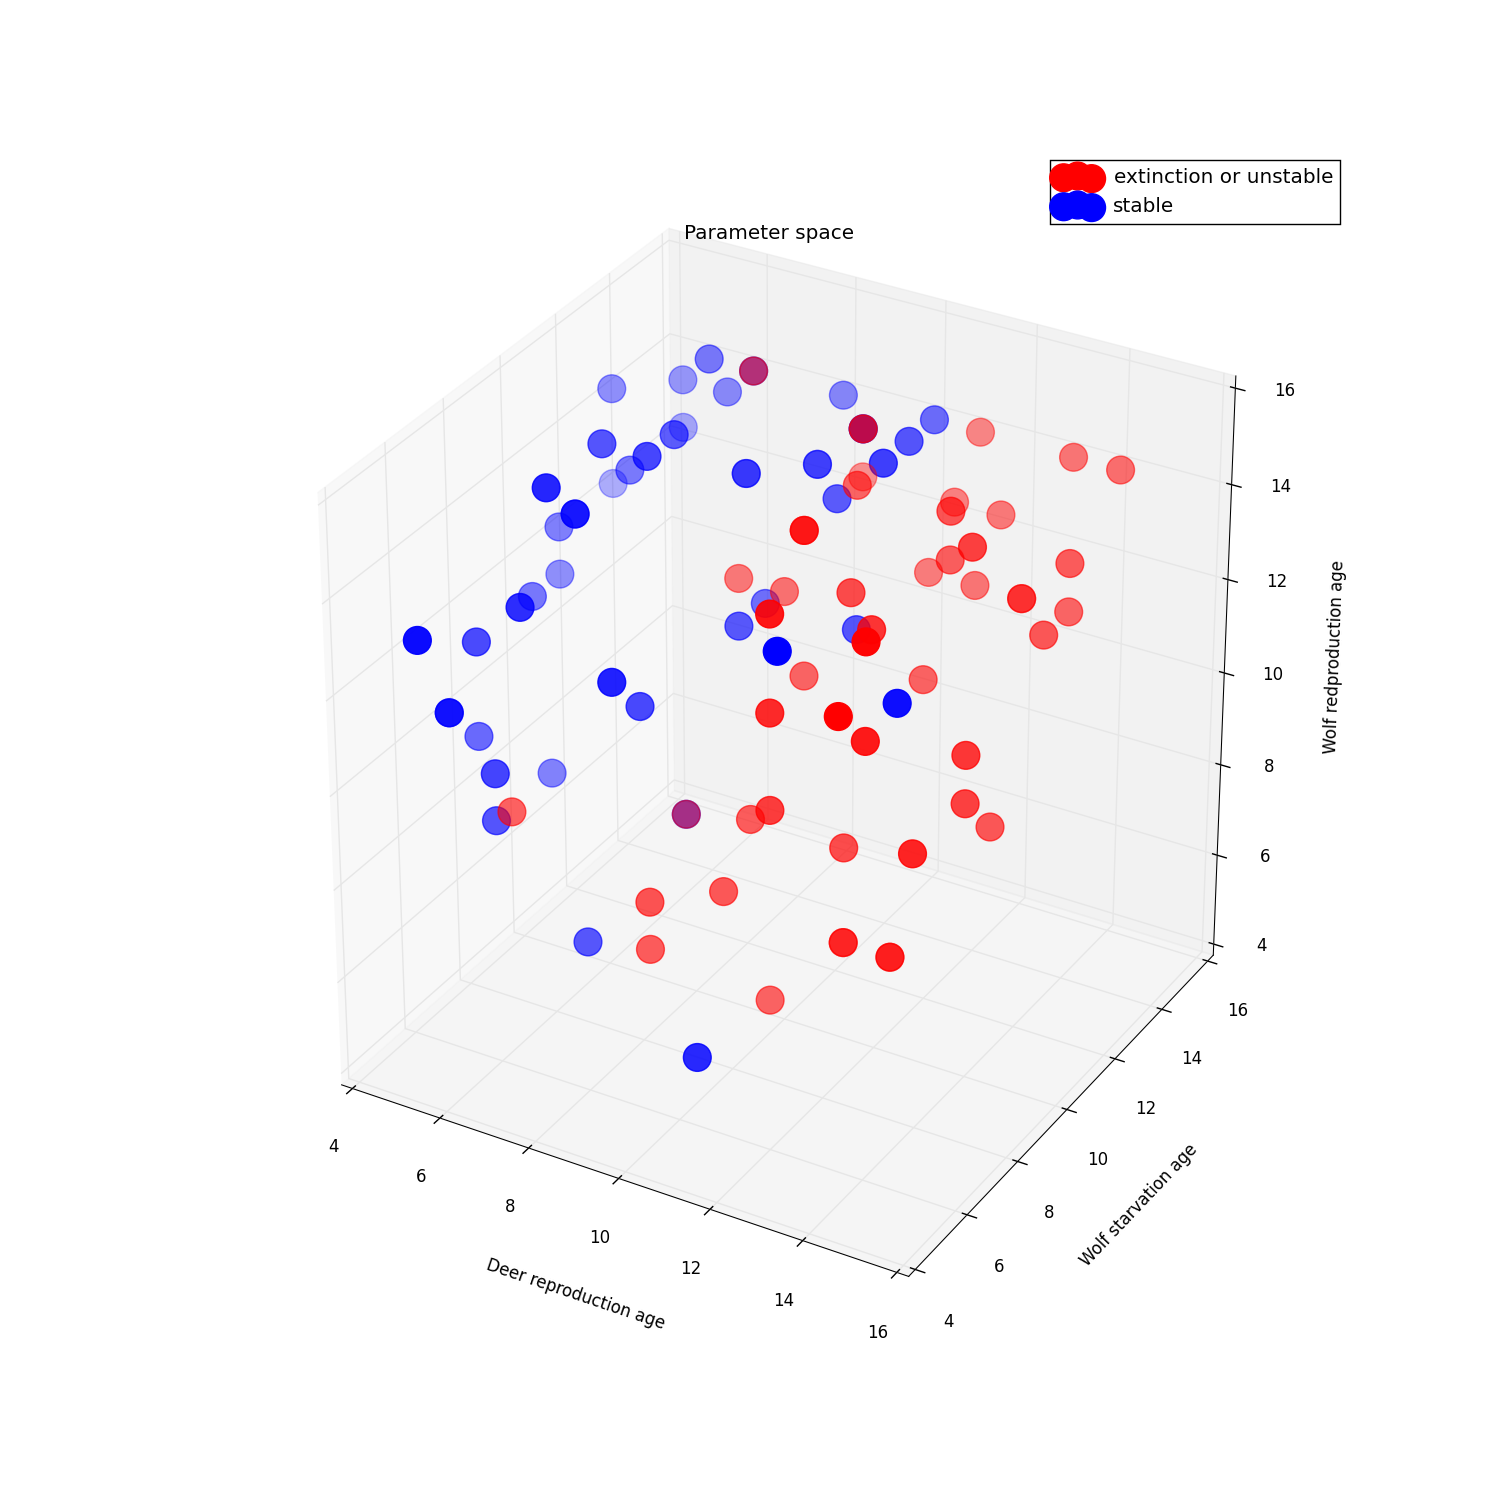
\includegraphics[width = 0.2\textwidth]{./pics/Restricted_Parameter_space_d250_w2500.png} \\
        \end{tabular}
        \label{RestrictParam}
  \end{figure}

}
\frame
{
	\frametitle{Population interaction of predator and prey in eco-system}

	\begin{figure}[htbp]
	\begin{center}
	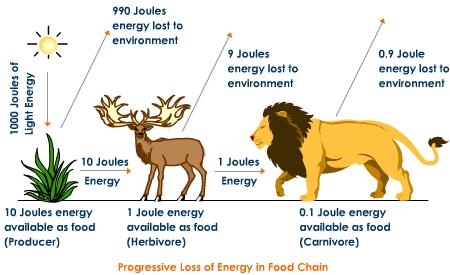
\includegraphics[width=1\textwidth]{./pics/progressive-energy-loss.jpeg}
	\caption{default}
	\label{default}
	\end{center}
	\end{figure}
}


\section{Results and discussion}
\frame
{
  \frametitle{Ecosystem at Equilibrium}
  Parameters used: 
  \begin{itemize}
  \item{Initial number of deer: 2,500}
  \item{Initial number of wolves: 250}
  \item{Deer reproduction rate: 5}
  \item{Wolf reproduction rate: 14}
  \item{Wolf starvation rate: 11}
  \end{itemize}
  \center{ Animation Time! }

}


\end{document}
